% "{'classe':('PSI'),'chapitre':'dyn_cin','type':('td'),'titre':'Régulateur centrifuge', 'source':'C. Gamelon et P. Dubois','comp':('C1-05','C2-09'),'corrige':True}"
%\setchapterimage{bandeau
\chapter*{Application \arabic{cptApplication} \\ 
Régulateur centrifuge -- \ifprof Corrigé \else Sujet \fi}
\addcontentsline{toc}{section}{Application \arabic{cptApplication} : Régulateur centrifuge -- \ifprof Corrigé \else Sujet \fi}

\iflivret \stepcounter{cptApplication} \else
\ifprof  \stepcounter{cptApplication} \else \fi
\fi

\setcounter{question}{0}
\marginnote{C. Gamelon \& P. Dubois.}
\marginnote[1cm]{
\UPSTIcompetence[2]{C1-05}
\UPSTIcompetence[2]{C2-09}
}
\begin{marginfigure}[4cm]
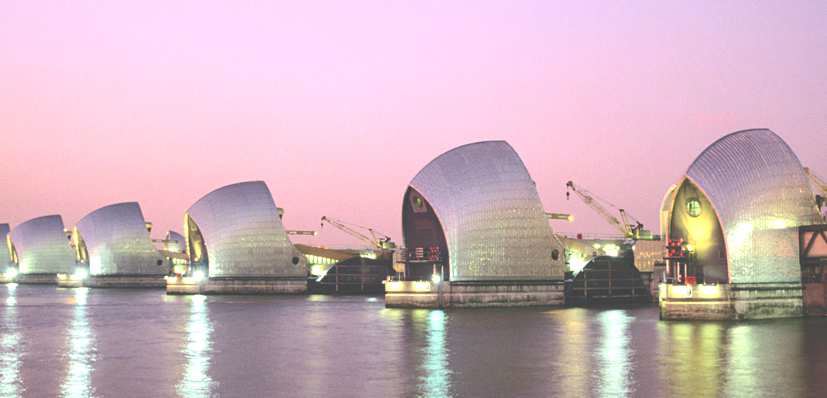
\includegraphics[width=\linewidth]{fig_00}
\end{marginfigure}


\begin{marginfigure}[10cm]
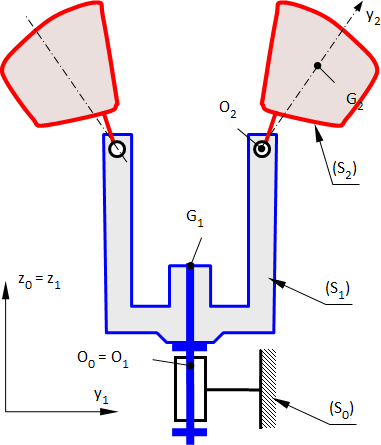
\includegraphics[width=\linewidth]{fig_02}
\end{marginfigure}

On considère le mécanisme de la figure ci-contre, qui représente le régulateur centrifuge utilisé dans la direction assistée << DIRAVI >> de CITROËN. Ce système, dont la fréquence de rotation est liée à la vitesse du véhicule, agit sur un circuit hydraulique et permet de faire varier l’assistance en fonction de la vitesse.
Considérons uniquement le rotor \textbf{($S_1$)} et la masselotte \textbf{($S_2$)} représentés schématiquement ci-contre.

\begin{multicols}{2}
\begin{itemize}
\item \textbf{($S_1$)} est en liaison pivot d'axe $\axe{O_1}{z_0}$ avec \textbf{($S_0$)}.
\item \textbf{($S_2$)} est en liaison pivot d'axe $\axe{O_2}{x_1}$ avec \textbf{($S_1$)}.
\item $\angl{x_0}{x_1} = \angl{y_0}{y_1}=\theta_1$.
\item $\angl{y_1}{y_2} = \angl{z_1}{z_2}=\theta_2$.
\item $\vect{O_0G_1}=h_1\vect{z_0}$.
\item $\vect{O_0O_2}=d_1\vect{z_0}+L_1\vect{y_1}$.
\item $\vect{O_2G_2}=L_2\vect{y_2}$.
\end{itemize}
\end{multicols}

Pour chacun des solides $S_i$ on note $m_i$ la masse, $\inertie{G_i}{S_i}=\matinertie{A_i}{B_i}{C_i}{-D_i}{-E_i}{-F_i}{B_i}$.

On note $E=\left\{ S_1,S_2\right\}$. 
Une vue 3D de la masselotte est donnée ci-dessous. 

\ifprof
\begin{center}
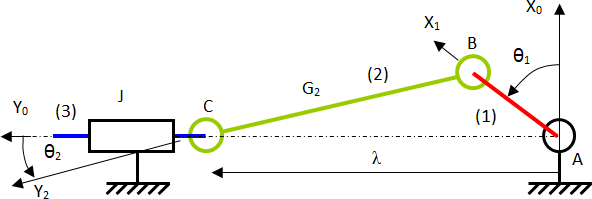
\includegraphics[width=.5\linewidth]{fig_03}
\end{center}
\else
\begin{center}
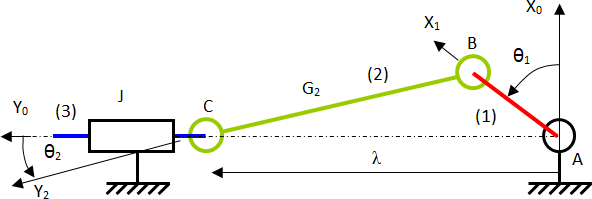
\includegraphics[width=.7\linewidth]{fig_03}
\end{center}
\fi

\question{Indiquer, sans développer de calculs, quelles sont les particularités des matrices d’inertie des solides (1) et (2).}
\ifprof
\begin{corrige}
Le solide 1 est axisymétrique. En tout point de l'axe du solide, la matrice d'inertie sera diagonale. On a donc $\inertie{O_1}{S_1}=\matinertie{A_1}{B_1}{C_1}{0}{0}{0}{B_1}$.

Le solide 2 admet le plan $\angl{y_2}{z_2}$ comme plan de symétrie. Les produits d'inertie dépendant de $x$ sont nuls. On a donc $\inertie{G_2}{S_2}=\matinertie{A_2}{B_2}{C_2}{-D_2}{0}{0}{B_2}$.

\end{corrige}
\else
\fi


Afin de moins alourdir les calculs, on suppose constantes les vitesse de rotation $\dot{\theta}_1$ et $\dot{\theta}_2$.

\question{Discuter de la pertinence de ces hypothèses. Vous pourrez éventuellement les remettre en cause. }

\question{Déterminer le torseur dynamique $\torseurdyn{S_1}{R_0}$ en $O_1$ et le torseur dynamique  $\torseurdyn{S_2}{R_0}$ en $O_2$.}

\ifprof
\begin{corrige}~\\


\begin{center}
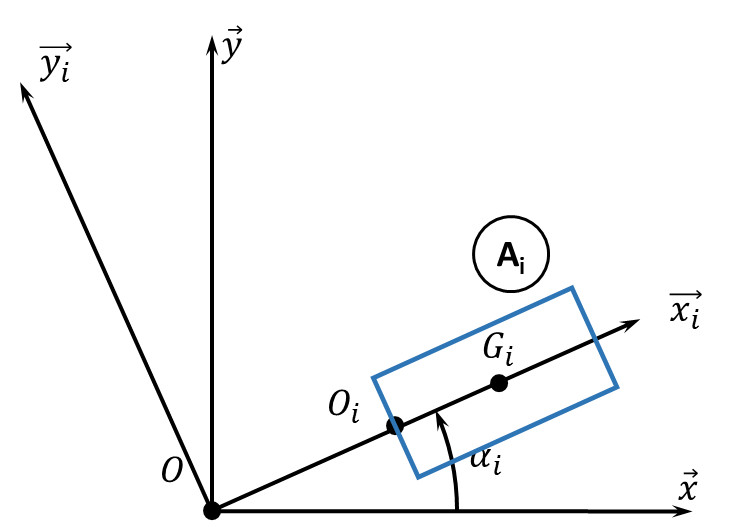
\includegraphics[width=.48\linewidth]{param.png}
\end{center}


\textbf{Mouvement du solide 1/0}

On a : 
$\torseurcin{V}{S_1}{R_0}=\torseurl{\dot{\theta}_1 \vect{z_1}}{\vect{0}}{G_1}=\torseurl{\dot{\theta}_1 \vect{z_1}}{\vect{0}}{O_1}$. 

$O_1$ est un point fixe dans $R_0$. 

$\torseurci{S_1}{R_0}
=\torseurl{
\vect{0}
}{
\inertie{O_1}{S_1}\vecto{S_1}{R_0}
}{O_1}
=\torseurl{
\vect{0}
}{
C_1\dot{\theta}_1\vect{z_1}
}{O_1}
$ 
et 
$\torseurdyn{S_1}{R_0}
=\torseurl{
\vect{0}
}{
C_1\ddot{\theta}_1\vect{z_1}
}{O_1}
.$

\textbf{Mouvement du solide 2/0}

On a : 
$\torseurcin{V}{S_2}{R_0}
=\torseurl{\dot{\theta}_1 \vect{z_1}+\dot{\theta}_2 \vect{x_2}}{\vectv{G_2}{S_2}{R_0}}{G_2}
=\torseurl{\dot{\theta}_1 \vect{z_1}+\dot{\theta}_2 \vect{x_2}}{
 L_2 \dot{\theta}_2 \vect{z_2}-\dot{\theta}_1L_1\vect{x_1}
}{G_2}$. 

$\vectv{G_2}{S_2}{R_0}=\vectv{G_2}{S_2}{S_1}+\vectv{G_2}{S_1}{R_0}$

$=
\left( \underbrace{\vectv{O_2}{S_2}{S_1}}_{\vect{0}}+\vect{G_2O_2}\wedge \vecto{S_2}{S_1}\right)
+ \left( \underbrace{\vectv{O_0}{S_1}{R_0}}_{\vect{0}}+\vect{G_2O_0}\wedge \vecto{S_1}{R_0}\right)$

$=
\left( -L_2\vect{y_2}\wedge \dot{\theta}_2 \vect{x_2}\right)
+ \left(-\left( d_1\vect{z_0}+L_1\vect{y_1}+L_2\vect{y_2} \right)\wedge \dot{\theta}_1 \vect{z_1}\right)$
$=
 L_2 \dot{\theta}_2 \vect{z_2}-
\dot{\theta}_1\left (L_1+L_2 \cos\theta_2 \right)\vect{x_1}
$

$G_2$ est le centre de gravité de $S_2$. 

$\torseurci{S_2}{R_0}
=\torseurl{
m_2\left(   L_2 \dot{\theta}_2 \vect{z_2}-\dot{\theta}_1\left (L_1+L_2 \cos\theta_2 \right)\vect{x_1}\right)
}{
\inertie{G_2}{S_2}\vecto{S_2}{R_0}
}{G_2}
%=\torseurl{
%\vect{0}
%}{
%%C_1\dot{\theta}_1\vect{z_1}
%}{G_2}
%$ 
%et 
%$\torseurdyn{S_2}{R_0}
%=\torseurl{
%\vect{0}
%}{
%%C_1\ddot{\theta}_1\vect{z_1}
%}{G_1}
%.
$

$\vecto{S_2}{R_0}
=\dot{\theta}_1 \vect{z_1}+\dot{\theta}_2 \vect{x_2}
=\dot{\theta}_1 \left( \cos\theta_2 \vect{z_2}+\sin\theta_2 \vect{y_2} \right)+\dot{\theta}_2 \vect{x_2}
$

$\inertie{G_2}{S_2}\vecto{S_2}{R_0}=
\matinertie{A_2}{B_2}{C_2}{-D_2}{0}{0}{B_2}
\begin{pmatrix}
\dot{\theta}_2 \\
\dot{\theta}_1\sin\theta_2\\
\dot{\theta}_1\cos\theta_2
\end{pmatrix}_{B_2}
=
\begin{pmatrix}
A_2\dot{\theta}_2 \\
B_2\dot{\theta}_1\sin\theta_2 - D_2 \dot{\theta}_1\cos\theta_2\\
-D_2\dot{\theta}_1\sin\theta_2 +C_2 \dot{\theta}_1\cos\theta_2
\end{pmatrix}_{B_2}
$

$\torseurdyn{S_2}{R_0}
=\torseurl{
m_2 \vectg{G_2}{S_2}{R_0}
}{
\left[\dfrac{\dd}{\dd t}\left(\inertie{G_2}{S_2}\vecto{S_2}{R_0}\right)\right]_{R_0}
}{G_2}
$

$\vectg{G_2}{S_2}{R_0}
=\left[\dfrac{\text{d}\left( L_2 \dot{\theta}_2 \vect{z_2}-
\dot{\theta}_1\left (L_1+L_2 \cos\theta_2 \right)\vect{x_1}\right)}{\dd t}\right]_{R_0}$

$=L_2 \ddot{\theta}_2 \vect{z_2}+L_2 \dot{\theta}_2 \left( \dot{\theta}_1 \sin\theta_2 \vect{x_{1,2}} -\dot{\theta}_2 \vect{y_2} \right)
-\ddot{\theta}_1\left (L_1+L_2 \cos\theta_2 \right)\vect{x_1}
-\dot{\theta}_1\left (-L_2 \dot{\theta}_2\sin\theta_2 \right)\vect{x_1}
-\dot{\theta}_1^2\left (L_1+L_2 \cos\theta_2 \right)\vect{y_1}$

$=L_2 \ddot{\theta}_2 \vect{z_2}-L_2 \dot{\theta}_2^2 \vect{y_2} 
+\left(2L_2 \dot{\theta}_1 \dot{\theta}_2 \sin\theta_2 %\vect{x_1}
-\ddot{\theta}_1\left (L_1+L_2 \cos\theta_2 \right)\right)\vect{x_1}
-\dot{\theta}_1^2\left (L_1+L_2 \cos\theta_2 \right)\vect{y_1}$


$\left[\dfrac{\dd}{\dd t}\inertie{G_2}{S_2}\vecto{S_2}{R_0}\right]_{R_0}=...$

$=
\begin{pmatrix}
A_2\ddot{\theta}_2 \\
B_2\ddot{\theta}_1\sin\theta_2 - D_2 \ddot{\theta}_1\cos\theta_2
+B_2\dot{\theta}_1\dot{\theta}_2\cos\theta_2 + D_2 \dot{\theta}_1\dot{\theta}_2\sin\theta_2\\
-D_2\ddot{\theta}_1\sin\theta_2 +C_2 \ddot{\theta}_1\cos\theta_2-D_2\dot{\theta}_1\dot{\theta}_2\cos\theta_2 -C_2 \dot{\theta}_1\dot{\theta}_2\sin\theta_2
\end{pmatrix}_{B_2}
$

$
+
A_2\dot{\theta}_2 \dot{\theta}_1 \vect{y_1}
+\left(B_2\dot{\theta}_1\sin\theta_2 - D_2 \dot{\theta}_1\cos\theta_2\right)\left( -\dot{\theta}_1 \cos\theta_2\vect{x_1}+\dot{\theta}_2 \vect{z_2}\right)
+\left(-D_2\dot{\theta}_1\sin\theta_2 +C_2 \dot{\theta}_1\cos\theta_2\right) \left( \dot{\theta}_1 \sin\theta_2 \vect{x_{1,2}} -\dot{\theta}_2 \vect{y_2} \right)
$



$\left[\dfrac{\text{d} \vect{z_2}}{\text{d} t}\right]_{R_0}
=\left[\dfrac{\text{d} \vect{z_2}}{\text{d} t}\right]_{R_2} + \vecto{S_2}{R_0}\wedge\vect{z_2}
= \left( \dot{\theta}_1 \vect{z_1}+\dot{\theta}_2 \vect{x_2}\right) \wedge \vect{z_2}
= \dot{\theta}_1 \sin\theta_2 \vect{x_{1,2}} -\dot{\theta}_2 \vect{y_2} 
$


$\left[\dfrac{\text{d} \vect{y_2}}{\text{d} t}\right]_{R_0}
=\left[\dfrac{\text{d} \vect{y_2}}{\text{d} t}\right]_{R_2} + \vecto{S_2}{R_0}\wedge\vect{y_2}
= \left( \dot{\theta}_1 \vect{z_1}+\dot{\theta}_2 \vect{x_2}\right) \wedge \vect{y_2}
= -\dot{\theta}_1 \cos\theta_2\vect{x_1}+\dot{\theta}_2 \vect{z_2}
$


$\left[\dfrac{\text{d} \vect{x_2}}{\text{d} t}\right]_{R_0}
=\left[\dfrac{\text{d} \vect{x_1}}{\text{d} t}\right]_{R_0}
=\left[\dfrac{\text{d} \vect{x_1}}{\text{d} t}\right]_{R_1} + \vecto{S_1}{R_0}\wedge\vect{x_1}
=\dot{\theta}_1 \vect{z_1} \wedge  \vect{x_1}
=\dot{\theta}_1 \vect{y_1}$

%=\torseurl{
%\vect{0}
%}{
%%C_1\dot{\theta}_1\vect{z_1}
%}{G_2}
%$ 
%et 
%$\torseurdyn{S_2}{R_0}
%=\torseurl{
%\vect{0}
%}{
%%C_1\ddot{\theta}_1\vect{z_1}
%}{G_1}
%.
%$



\end{corrige}
\else
\fi


\question{Déterminer $\vectmd{O_2}{2}{0}\cdot \vect{x_2}$.}
\ifprof
\begin{corrige}


$\vectmd{O_2}{2}{0}\cdot \vect{x_2}$

$= \left( \vectmd{G_2}{2}{0}+\vect{O_2G_2}\wedge M_2\vectg{G_2}{2}{0}\right)\cdot \vect{x_2}$

$= \left( \left[\dfrac{\dd}{\dd t}\inertie{G_2}{S_2}\vecto{S_2}{R_0}\right]_{R_0}
+\vect{O_2G_2}\wedge M_2\vectg{G_2}{2}{0}\right)\cdot \vect{x_2}$

$\left[\dfrac{\dd}{\dd t}\inertie{G_2}{S_2}\vecto{S_2}{R_0} \cdot \vect{x_2} \right]_{R_0}
=\left[\dfrac{\dd}{\dd t}\inertie{G_2}{S_2}\vecto{S_2}{R_0}  \right]_{R_0}\cdot \vect{x_2}+\left[\dfrac{\dd}{\dd t}\inertie{G_2}{S_2}\vecto{S_2}{R_0} \cdot \vect{x_2} \right]_{R_0}$
\end{corrige}
\else
\fi
%Q3- Calculer les composantes de la matrice
%du solide (2) au point G2.


\ifprof
\else
\begin{marginfigure}
\centering

\includegraphics[width=3cm]{Cy_04_02_Application_01_Regulateur_Diravi_qr}
\end{marginfigure}
\fi


\question{Comment pourrait-on déterminer le torseur dynamique  $\torseurdyn{E}{R_0}$ en $O_2$ ?}

\question{Donner une méthode qui permettrait d'obtenir le couple moteur nécessaire à la mise en mouvement du régulateur.}

\begin{marginfigure}
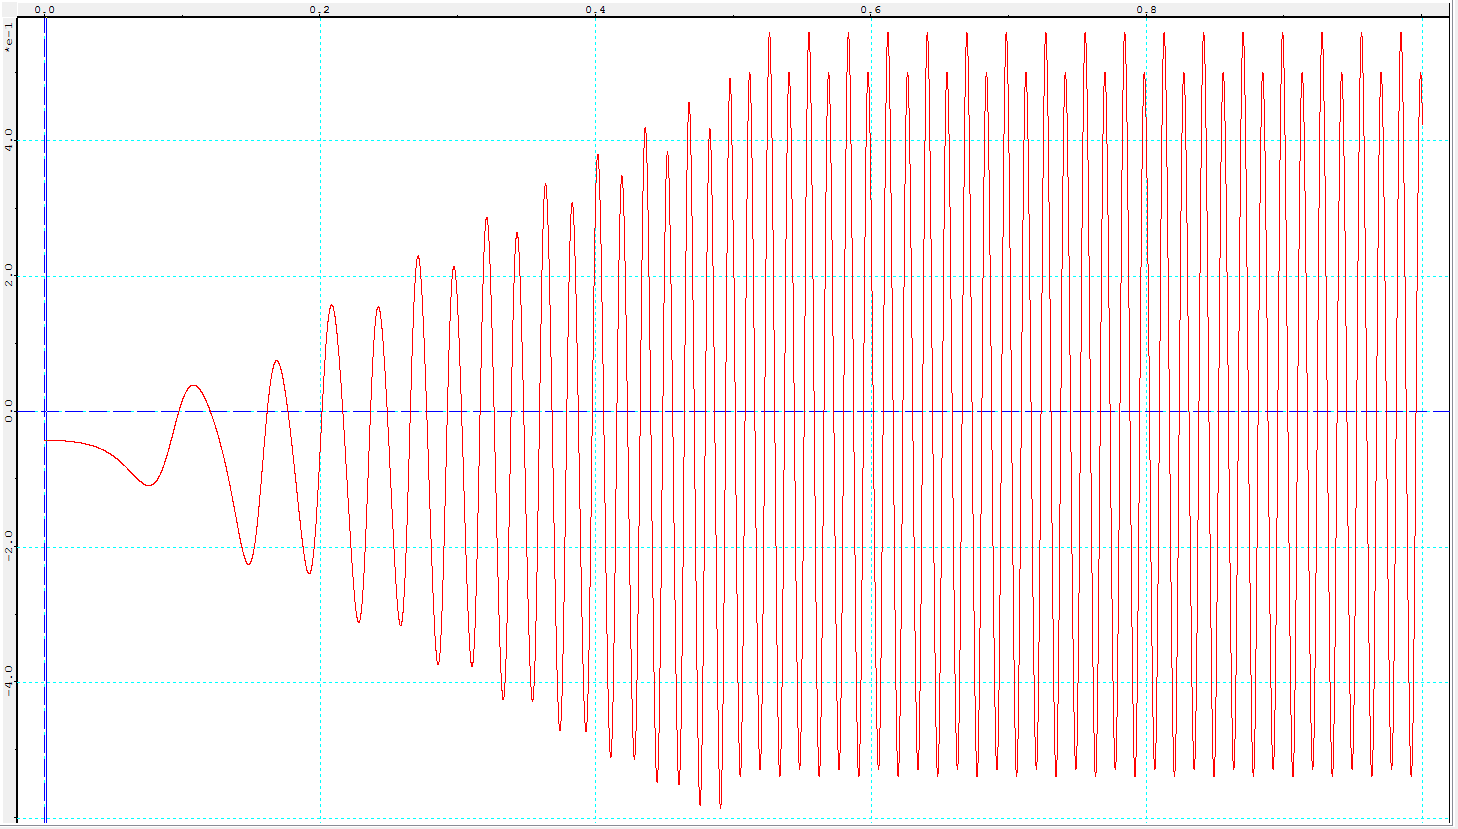
\includegraphics[width=\linewidth]{Cm_SansFrottement.png}
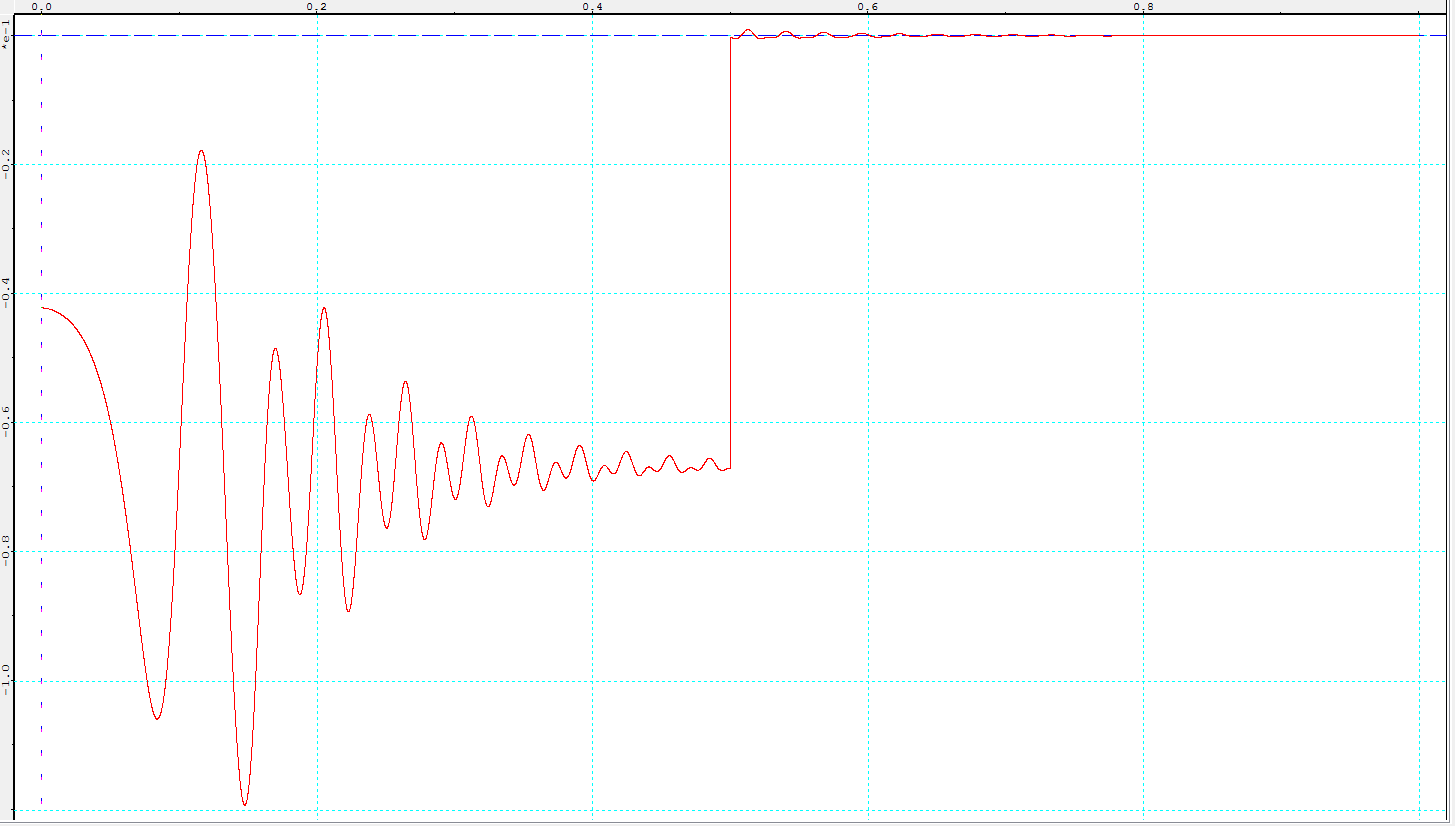
\includegraphics[width=\linewidth]{Cm_Frottement.png}
\end{marginfigure}

Pour mettre en mouvement le régulateur on réalise une montée en vitesse de 0 à 2000 tours par minute en 0,5 seconde.  On reste ensuite à vitesse constante. On donne le résultats de deux simulation permettant de calculer le couple nécessaire à la mise en mouvement du régulateur: la première sans frottement dans la liaison entre $S_1$ et $S_2$ (couple maximal \SI{0,46}{Nm}) , une seconde avec frottement (couple maximal \SI{0,1}{Nm}). 

\question{Commenter ces résultats. }




%\newpage

